\section{Robotics \& Non-Rigid Objects}
\frame{
  \frametitle{An Adaptive Robotic System for Doing Pick and Place Operations with Deformable Objects}
  Troels Bo Jørgensen, Sebastian Nesgaard Jensen, Henrik Aanæs, Niels Worsøe Hansen and Nobert Krüger

  \textit{Robotics and Computer-Integrated Manufacturing (Under review, Accepted)}
  \begin{figure}
    \centering
    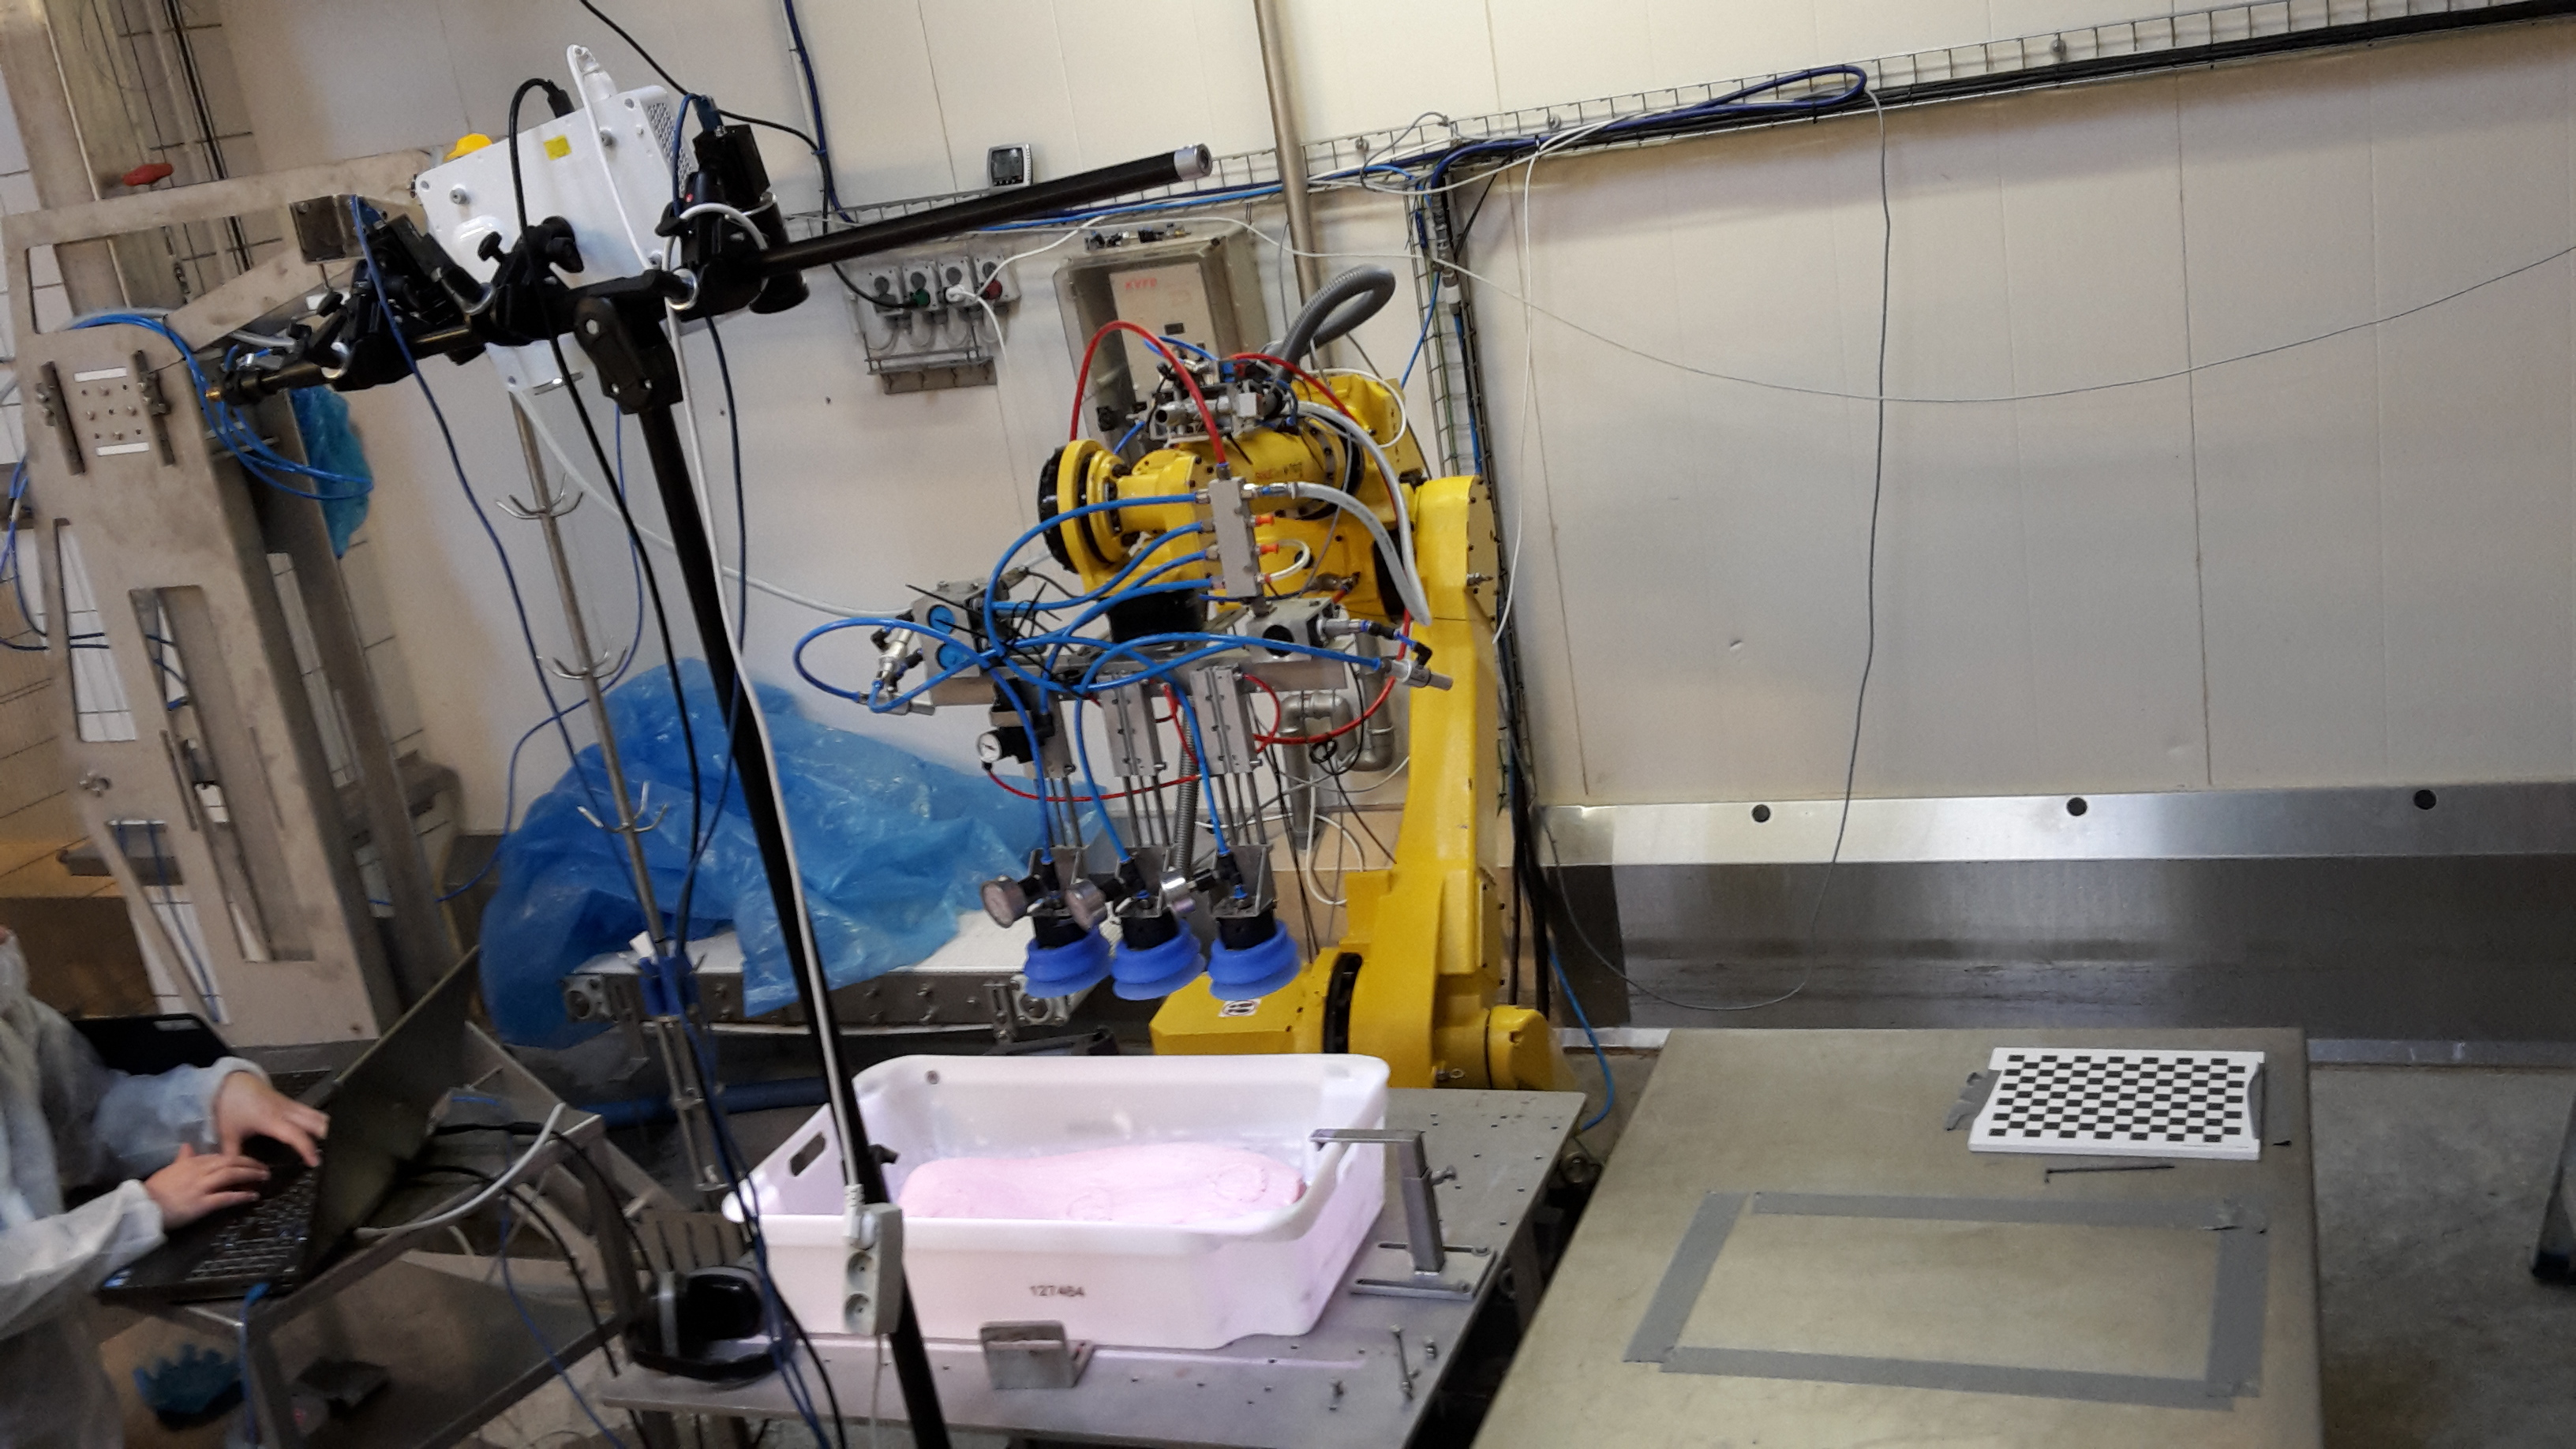
\includegraphics[height=0.65\textheight]{figures/dc_robot}
  \end{figure}
}

\frame{
  \frametitle{The Problem}
  \begin{minipage}{0.45\textwidth}
    \begin{itemize}
      \item Disorganized pile of deformable objects.
      \item Automatic pick and place operation.
      \item Focus on Danish Crown's meat packaging.
    \end{itemize}
  \end{minipage}
  \hfill
  \begin{minipage}{0.45\textwidth}
    \begin{figure}
      \centering
      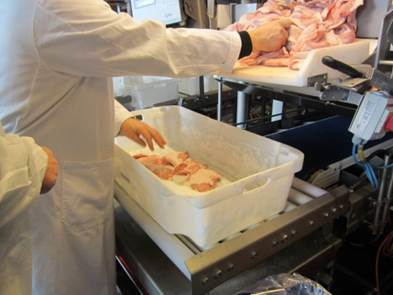
\includegraphics[width=\linewidth]{figures/dc_meatmanual}
    \end{figure}
  \end{minipage}
}

\frame{
  \frametitle{Why 3D?}
  \begin{center}
    \begin{itemize}
      \item Suction cups MUST be placed perpendicularly.
      \item Physical extent needed for placement calculations.
      \item Depth makes segmentation easier.
      \item Avoid areas with high curvature.
    \end{itemize}
  \end{center}
}

\frame{
  \frametitle{Phase-Shifting Structured Light}
  \begin{minipage}{0.55\textwidth}
    Fine-grained pattern,
    \begin{align*}
      p_{K, n}(u, v) = \frac{1}{2} + \frac{1}{2}\cos\left(2\pi\left(\frac{n}{N} + uK\right)\right),
    \end{align*}
    where $K$ is the number of spatial periods and $n$ is the pattern number.

    Use global unwrapper to determine $K$.
  \end{minipage}
  \begin{minipage}{0.4\textwidth}
    \begin{figure}
      \includegraphics[width=0.9\linewidth]{figures/ps_multi_phase}
    \end{figure}
  \end{minipage}
}

\frame{
  \frametitle{Guidance using Structured Light Scanning}
  \begin{figure}
    \centering
    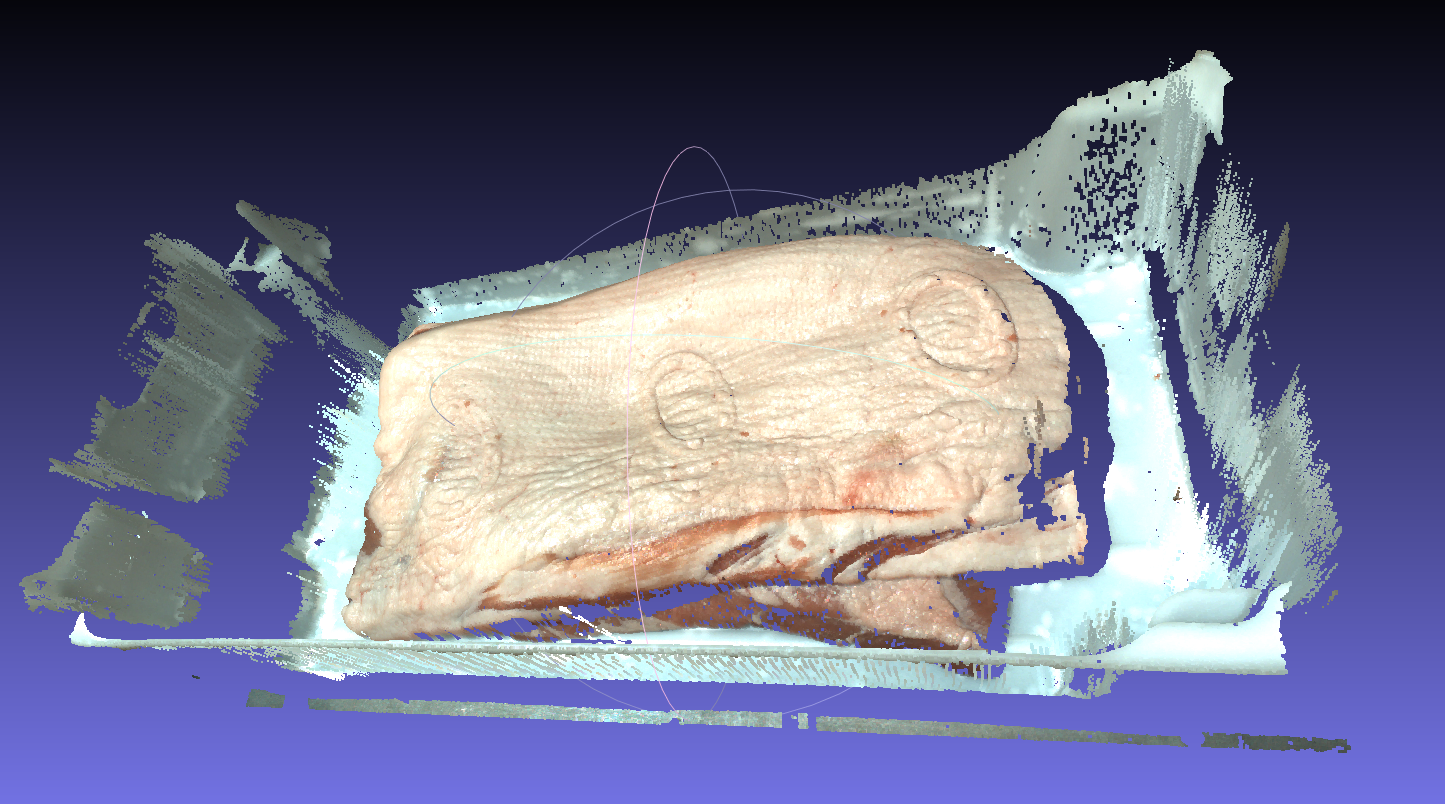
\includegraphics[height=0.6\textheight]{figures/dc_cloud}
    \hfill
    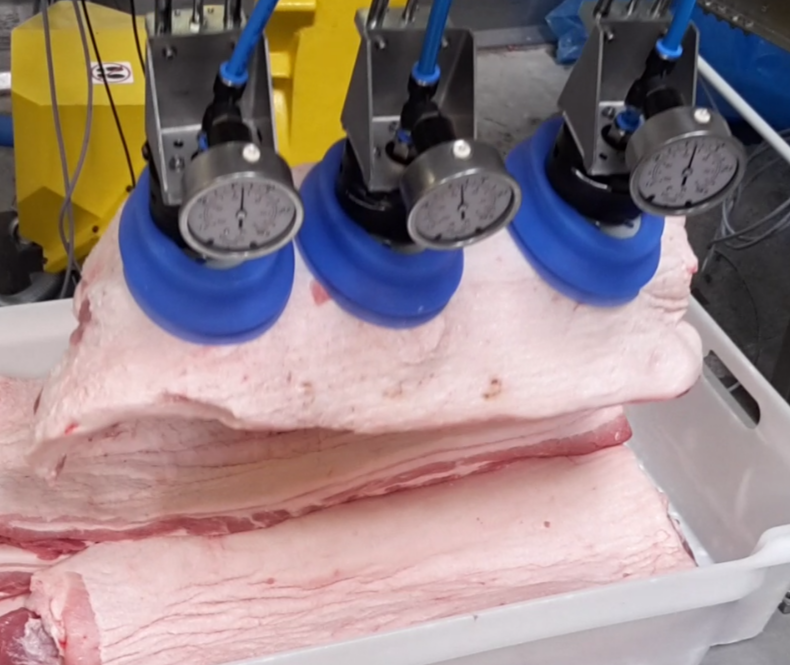
\includegraphics[height=0.6\textheight]{figures/dc_lift}
  \end{figure}
}

\frame{
  \frametitle{Segmentation}
  \begin{minipage}{0.45\textwidth}
    \begin{itemize}
      \item Region growth.
      \item Seeds at points of low curvature.
      \item Growth terminates at high curvature or normal angles.
      \item Neighborhood searches in imagespace.
    \end{itemize}
  \end{minipage}
  \hfill
  \begin{minipage}{0.45\textwidth}
    \begin{figure}
      \centering
      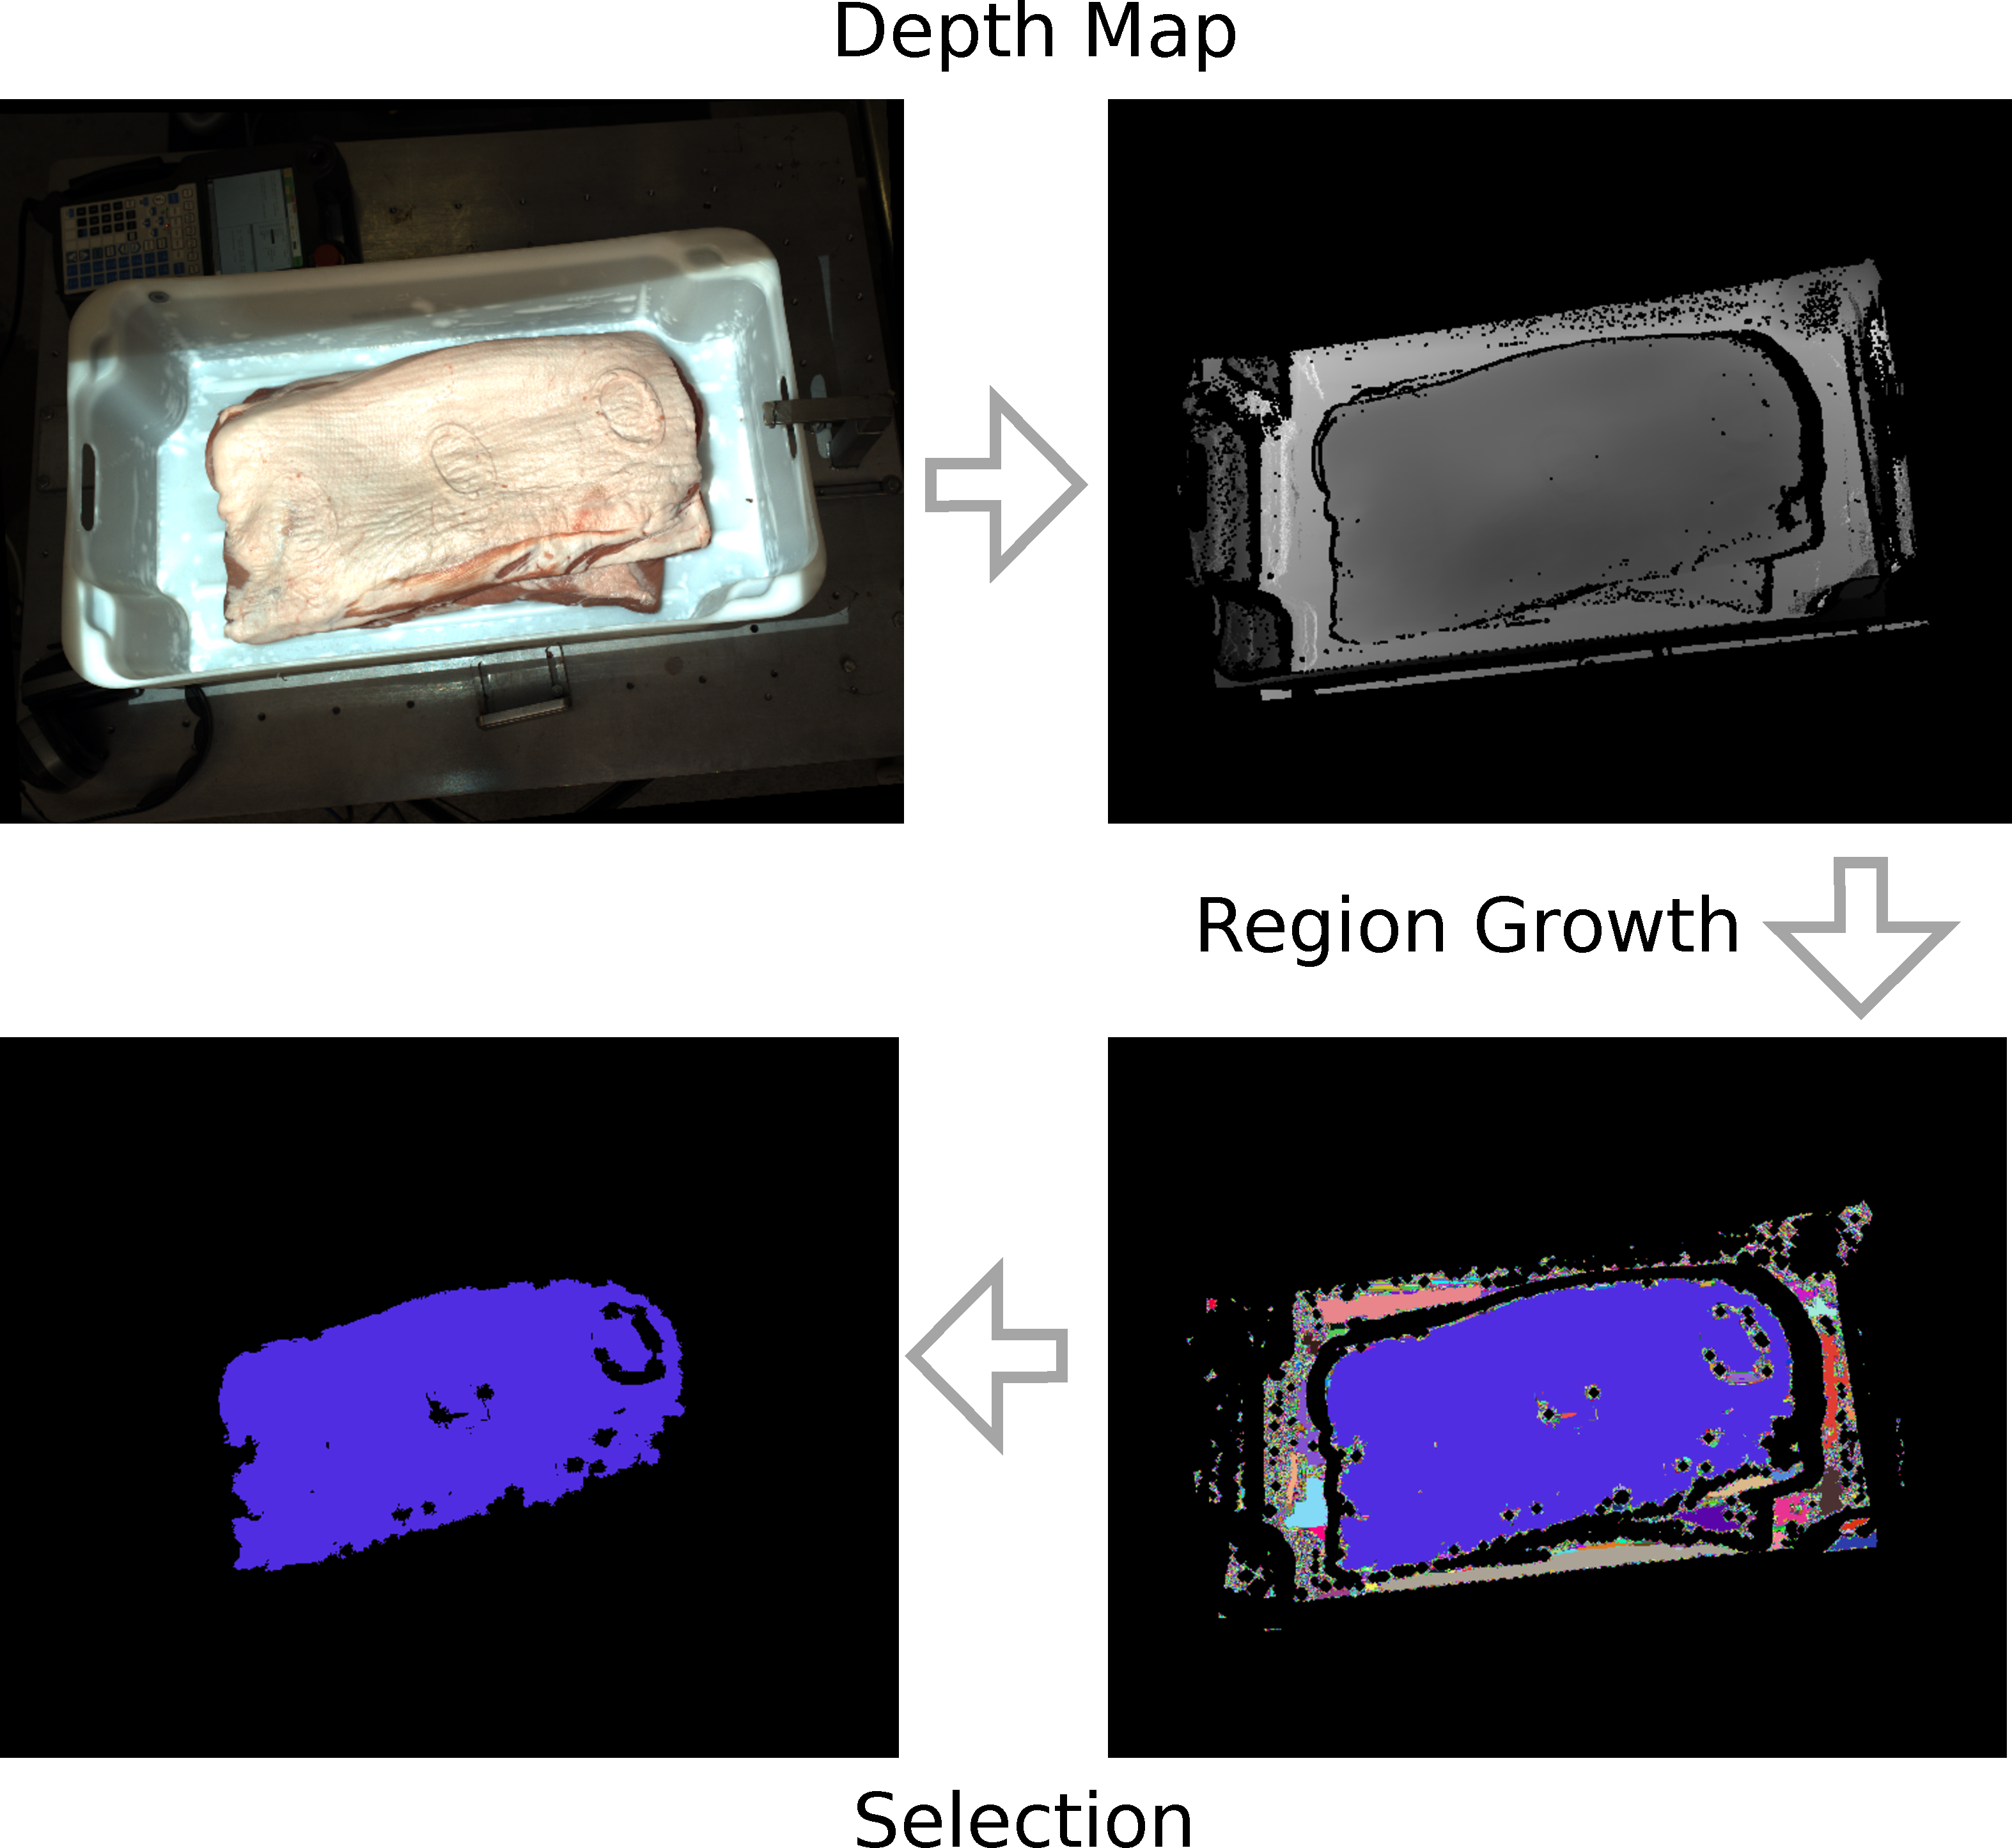
\includegraphics[height=0.8\textheight]{figures/dc_seg}
    \end{figure}
  \end{minipage}
}

\begin{comment}

\frame{
  \frametitle{Why no CNNs?}
  \begin{itemize}
    \item Need to run in real-time on a laptop CPU.
    \item Not much time for training data collection and labelling.
  \end{itemize}
}

\end{comment}

\frame{
  \frametitle{Demonstration}
  \setlength{\dcwidth}{720px}
  \setlength{\dcheight}{480px}
  \begin{center}
    %\movie[showcontrols, width = 1.35\textheight, height = 0.9\textheight, poster]{}{videos/succesDCManip.avi}
    \href{run:videos/succesDCManip.avi?autostart&loop}{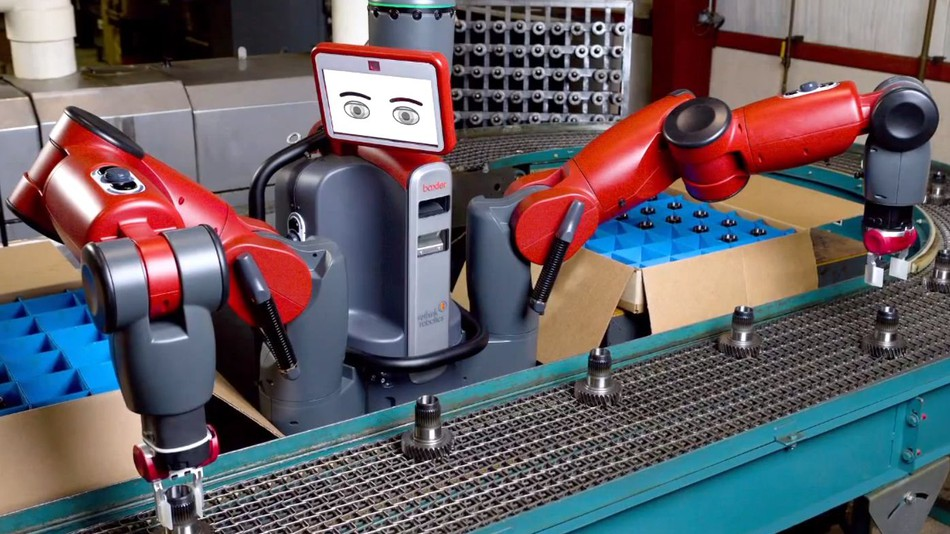
\includegraphics[width=0.4\dcwidth, height=0.4\dcheight]{figures/baxter.jpg}}
  \end{center}
}

\frame{
  \frametitle{Conclusion}
  \begin{itemize}
    \item Pick and place with deformable objects.
    \item Guidance using structured light.
    \item Working prototype demonstrated at Danish Crown, Ringsted.
    \item ROS for IPC and process-level parallelization.
  \end{itemize}
  \pnote{Time = 20m}
}
